\chapter{Evaluation}
\label{chap:evaluation}

% [Benchmarks tonen en bespreken van het lezen van de temperatuur native vs in Wasm. Het is niet de bedoeling om de runtimes te benchmarken.]

% Kunnen het zien als een tweeluik:
% 1. Functionele evaluatie: Werkt het?
% 2. Niet-functionele evaluatie: Performantie

% Dit kan op twee manieren gestructureerd worden:
% - Per implementatie zeggen of het werkt en performant is
% - Eerst werkt het, alle setups overlopen en dan overzichtsgrafiekje geven
% 	- Deze manier heeft Merlijns voorkeur omdat je zo mooi meer meta kunt gaan

\section{Evaluation setup}

The evaluation setup is based upon the setups used for the implementations, as shown in Chapter~\ref{chap:implementation}. It consists of the following:

\begin{itemize}
  \item A Raspberry Pi 4 Model B with 8 GB of RAM hooked up with a 4-digit 7-segment LED
  \item A Raspbery Pi 3 Model B with an attached HTS221 sensor
\end{itemize}

The display is evaluated natively and with Wasmtime and \gls{WAMR} as a runtime. The sensor will be evaluated in the same manner, but without the WAMR runtime.

The execution time is measured with the \texttt{criterion.rs} crate~\cite{gh:criterion}. This crate performs a hundred measurements, each containing many iterations of a routine, and then accumulates this into a probability density function. It indicates the estimated probability of an iteration taking a certain amount of time. Furthermore, the plot also contains a vertical line, this indicates the mean execution time. Thanks to the immense range of factors that can influence the execution time, outliers will always occur, and the resulting density functions aren't set in stone. Due to these outliers, sometimes a smaller extra peak can appear. Before measuring, Criterion first performs a warmup phase. Here, the routine is executed repeatdly to give the system time to adapt to the new workload. This helps prevent things like cold caches.

For memory profiling, \texttt{dhat-rs}~\cite{gh:dhat} is used. The profiler makes use of a global allocator that tracks allocations and deallocations on the heap. After execution, the total number of bytes, the maximum amount and the size at the end is printed. Together with the number of allocations.

The \texttt{flamegraph} crate~\cite{gh:flamegraph} is used to provide an in-depth overview of the functions an implementation uses under the hood. This overview is provided in fashion of flamegraphs. Many times per second, the threads in a program are interrupted and the current location in the code is recorded, along with the chain of functions that were called to get there. These samples are then processed and stacks that share common functions are added together. Then a figure is generated showing the call stacks that were measured. The x-axis doesn't show the passing of time. The left to right ordering has no meaning. The width of each block shows the total time that that function is on the CPU. A wider block means that it consumes more CPU per execution than other functions, or that it's called more. Each block's color is chosen at random.

% The implementations have the capabilities to write to a display and read from a sensor on two different runtimes, Wasmtime and WAMR. These both run on a Raspberry Pi, Wasmtime on Pico is not currently possible, and the WAMR build for the Pico fails at the linking stage.

\section{Functional evaluation}

This dissertation evaluates the applications on their execution time and used memory compared between running natively versus inside the Wasmtime and \gls{WAMR} runtimes. 

For this, two scenarios are tested:

\begin{itemize}
  \item On the Raspberry Pi 3 the temperature gets read out. This value is manually verified with the native implementation.
  \item On the Raspberry Pi 4 the string \texttt{"1234"} gets written to the display. This is visually verified, see Figure~\ref{fig:verif}.
\end{itemize}
% Voor de functionele evaluatie zijn er drie scenarios die getest worden.
% - Op de pico spreken we display X en tonen we daar Y, waarna het programma afsluit. we confirmeren visueel dat het getoond wordt. (foto van display)
% - Op de raspberry pi 3 wordt temperatuur uitgelezen. Temperatuur wordt manueel gecontroleerd met native programma.
% - Op raspberry pi 4.

\begin{figure}[h]
  \centering
  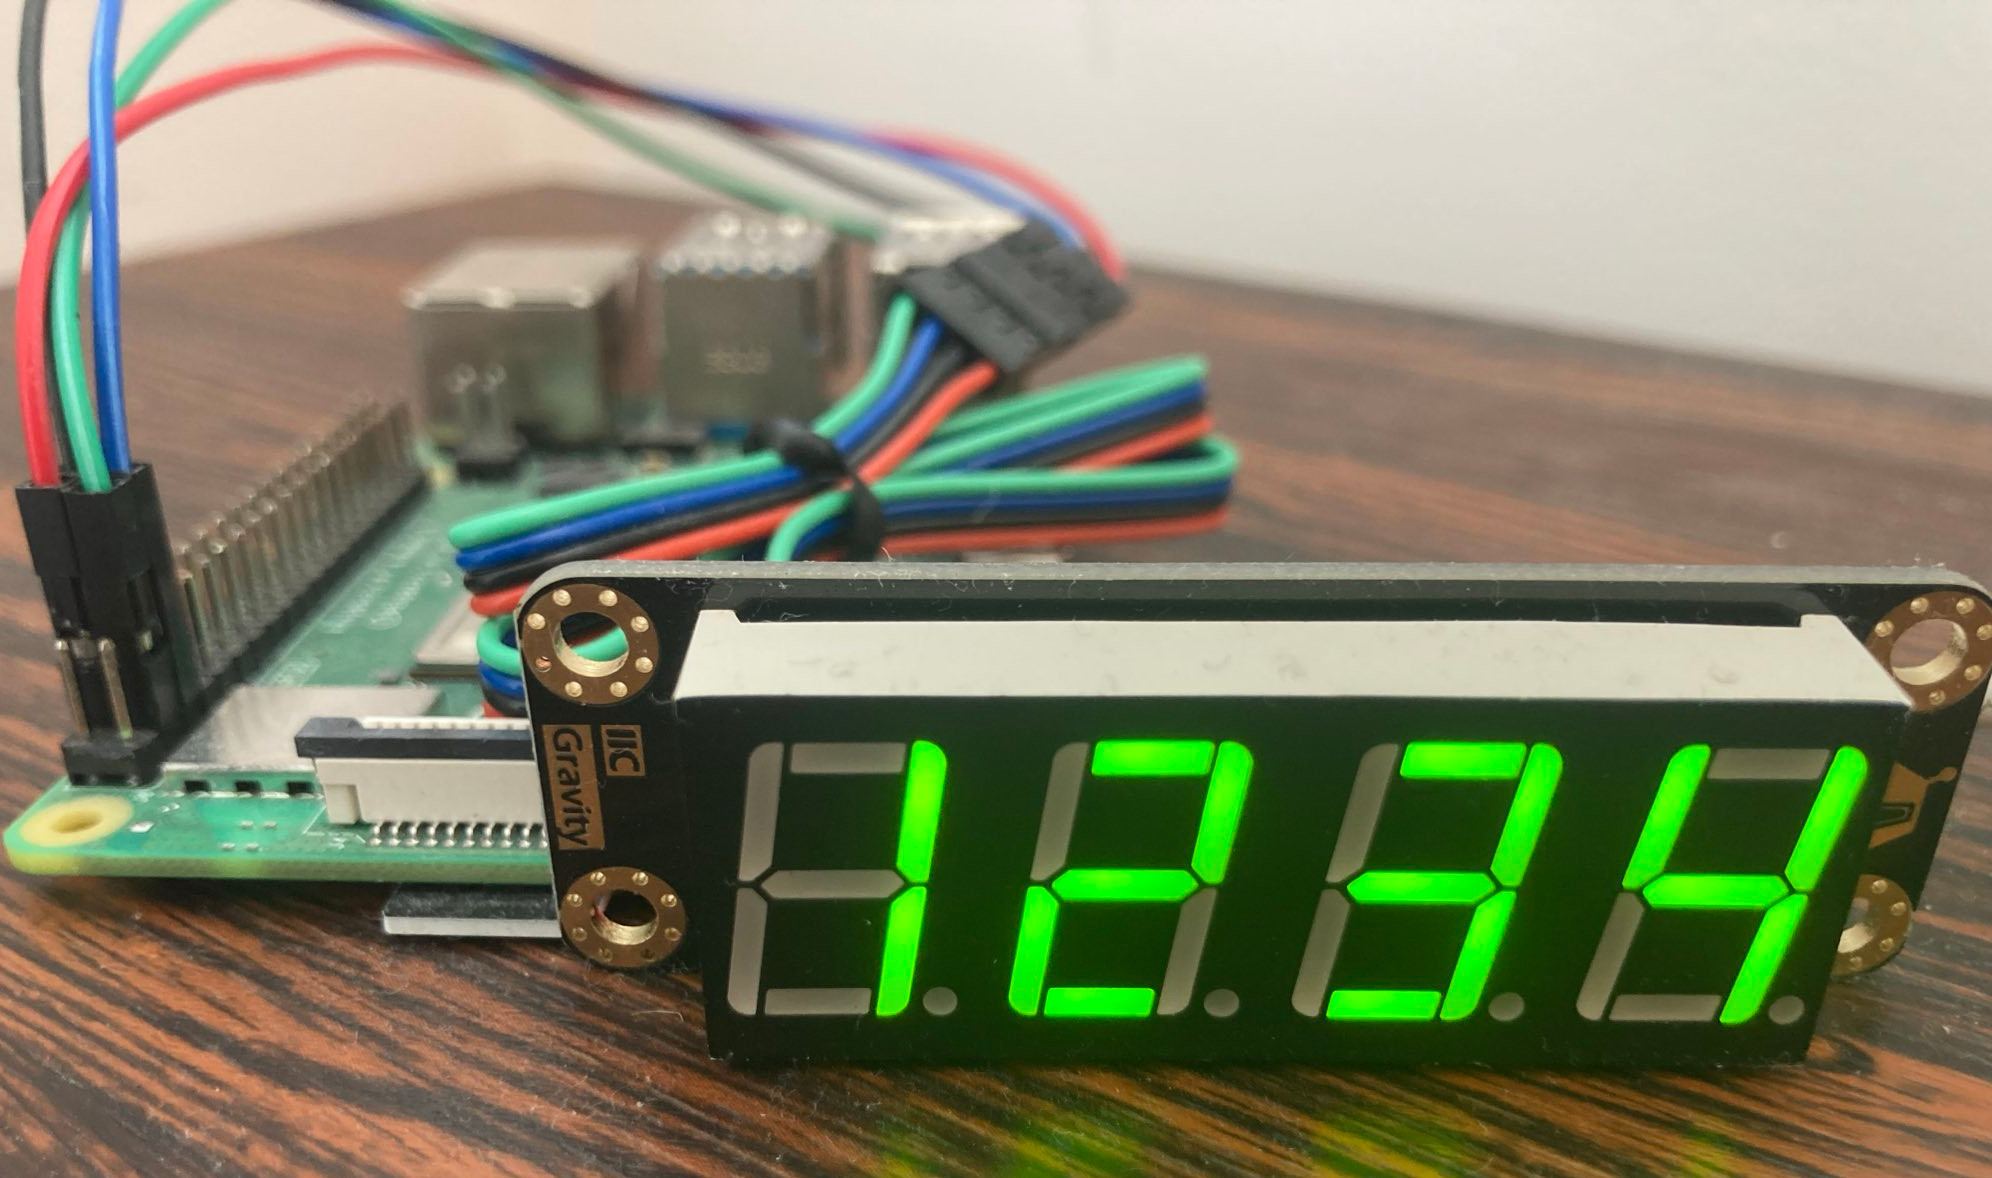
\includegraphics[width=0.5\textwidth]{figures/verification}
  \caption{Visual verification of the display}
  \label{fig:verif}
\end{figure}


% deze testen gedaan, dit is wat we willen
% werkt het?

\section{Benchmarks}

It is expected that running in Wasmtime will perform worse due to the imposed overhead on both execution time and memory usage, but that this overhead will be negligible. For WAMR, an even slimmer overhead is expected.

First, the execution time is inspected.
Both Figure~\ref{fig:sensor} and Figure~\ref{fig:display} showcase an astonishing longer execution time when running inside Wasmtime. The flamegraph in Figure~\ref{fig:flamegraph:wasmtime} gives the probable explanation, namely writing to the display is done inside the \texttt{\_start} block, almost all the other blocks are related to Cranelift.

Bytecode Alliance's Cranelift is a compiler backend that is among others in use by Wasmtime for just-in-time and ahead-of-time compilation. Via its ahead-of-time functionality, it is possible to greatly reduce the average execution time. There are two options to make use of this, through \texttt{wasmtime compile} or the \path{Component::serialize} function inside Wasmtime. To load such a precompiled file, the \path{Component::deserialize_file} function needs to be used, instead of \path{Component::from_file}. This file contains native, non-portable binary code which will not work on a different architecture, and might not even work across different processor models within the same architecture. Thus, it is not feasible to distribute a precompiled \gls{Wasm} binary, instead of the \gls{Wasm} binary itself\footnote{Technically, it is possible, but this requires careful configuration and is too complex for this dissertation.}.

\begin{figure}[h]
\centering
\begin{subfigure}{.5\textwidth}
  \centering
  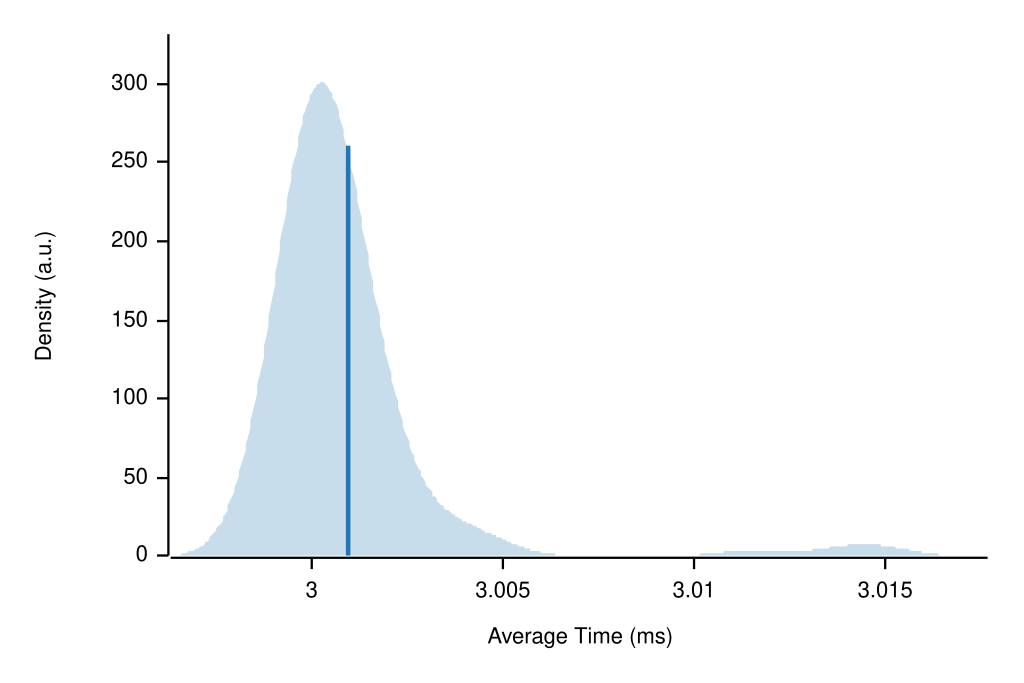
\includegraphics[width=\linewidth]{figures/native_led}
  \caption{Native}
  \label{fig:native_led}
\end{subfigure}%
\begin{subfigure}{.5\textwidth}
  \centering
  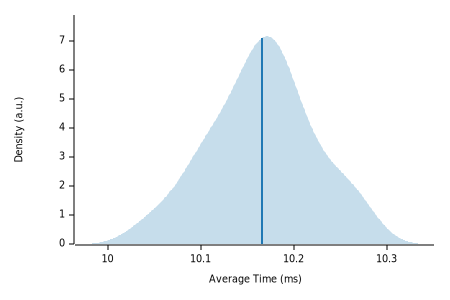
\includegraphics[width=\linewidth]{figures/wasmtime_led}
  \caption{Inside Wasmtime}
  \label{fig:wasmtime_led}
\end{subfigure}

\begin{subfigure}{.5\textwidth}
  \centering
  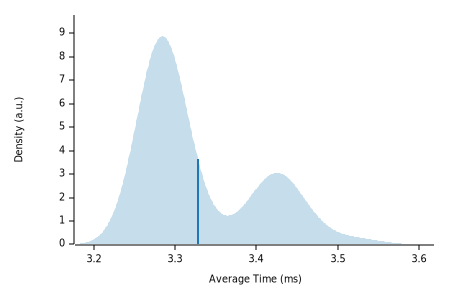
\includegraphics[width=\linewidth]{figures/compiled_led}
  \caption{Inside Wasmtime (precompiled)}
  \label{fig:led:compiled}
\end{subfigure}%
\begin{subfigure}{.5\textwidth}
  \centering
  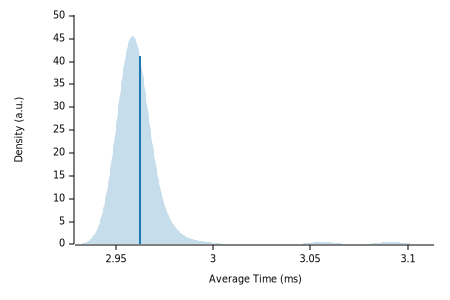
\includegraphics[width=\linewidth]{figures/optim_compiled_led}
  \caption{Inside Wasmtime (precompiled \& no command world)}
  \label{fig:led:wasmtime}
\end{subfigure}

\caption{Probability density function of execution time when writing to the display on....}
\label{fig:display}
\end{figure}

\begin{figure}[h]
\centering
\begin{subfigure}{.5\textwidth}
  \centering
  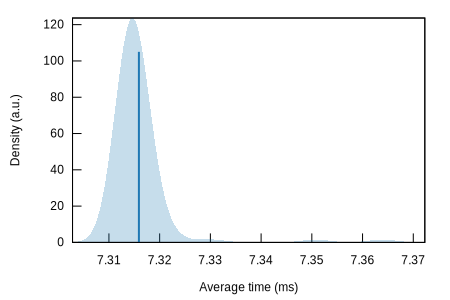
\includegraphics[width=\linewidth]{figures/native_hat_2}
  \caption{Native}
  \label{fig:native_hat}
\end{subfigure}%
\begin{subfigure}{.5\textwidth}
  \centering
  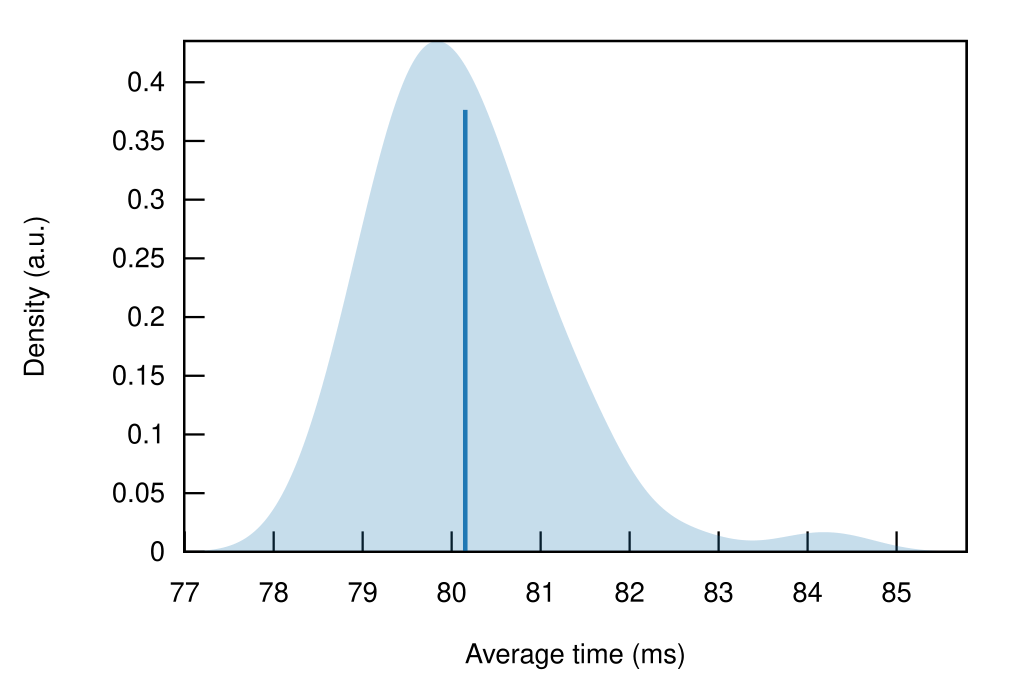
\includegraphics[width=\linewidth]{figures/wasmtime_hat}
  \caption{Inside Wasmtime}
  \label{fig:wasmtime_hat}
\end{subfigure}

\begin{subfigure}{.5\textwidth}
  \centering
  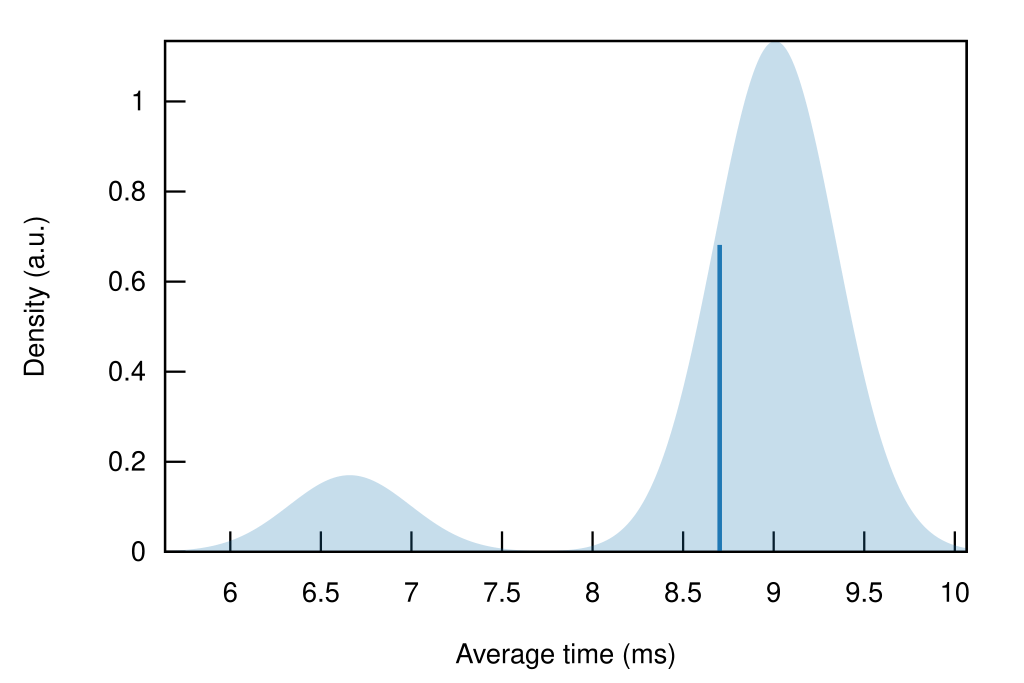
\includegraphics[width=\linewidth]{figures/compiled_hat}
  \caption{Inside Wasmtime (precompiled)}
  \label{fig:hat:compiled}
\end{subfigure}%
\begin{subfigure}{.5\textwidth}
  \centering
  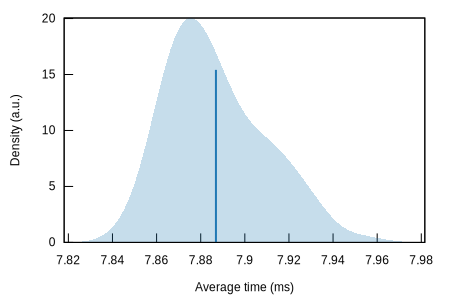
\includegraphics[width=\linewidth]{figures/optim_compiled_hat}
  \caption{Inside Wasmtime (precompiled \& no command world)}
  \label{fig:hat:wasmtime}
\end{subfigure}%

\caption{Probability density function of execution time when reading from the sensor on....}
\label{fig:sensor}
\end{figure}

Figure~\ref{fig:led:compiled} shows the execution time with a precompiled binary. It now is far more comparable to the average time of the native execution, with only an estimated slower mean run time of 0.3062 milliseconds. The same holds true for reading the sensor, Figure~\ref{fig:hat:compiled}, where the slowdown is now merely 1.3859 milliseconds. But, when compared to the experienced slowdown of the display implementation, this is still too much. The flamegraph inside Figure~\ref{fig:flamegraph:sensor} shows that nearly 14\% of the time is spent with adding the command world to the linker, using the \texttt{command::sync::add\_to\_linker} function, while this world technically isn't needed because of the custom host setup. Without this world, reading the sensor in Wasmtime is now only 0.571 milliseconds slower, Figure~\ref{fig:hat:wasmtime}, and writing to the display is 38.6 microseconds faster than native, Figure~\ref{fig:led:wasmtime}. The executed functions, see Figure~\ref{fig:flamegraph:led:native} and Figure~\ref{fig:flamegraph:led:compiled}, do not show any prominent differences. Thus, the speedup could be due to noise or kernel intrinsics.

\begin{figure}
  \centering
  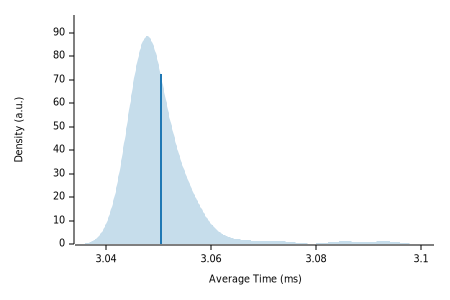
\includegraphics[width=0.5\textwidth]{figures/wamr_led}
  \caption{Probability density function of the execution time when writing to the display inside WAMR}
  \label{fig:led:wamr}
\end{figure}


Comparing WAMR with the fastest Wasmtime version for writing to the display, thus Figure~\ref{fig:led:wamr} with \ref{fig:led:wasmtime}, shows that Wasmtime outperforms with 88.2 microseconds. This is not significant enough of a difference for one to be faster or slower than the other. Looking at the flamegraph for WAMR, Figure~\ref{fig:flamegraph:led:wamr}, it is apparant that a considerable amount of time is spent on a page translation fault. 

% TODO: Grafiek voor sensor read
\begin{figure}
  \centering
  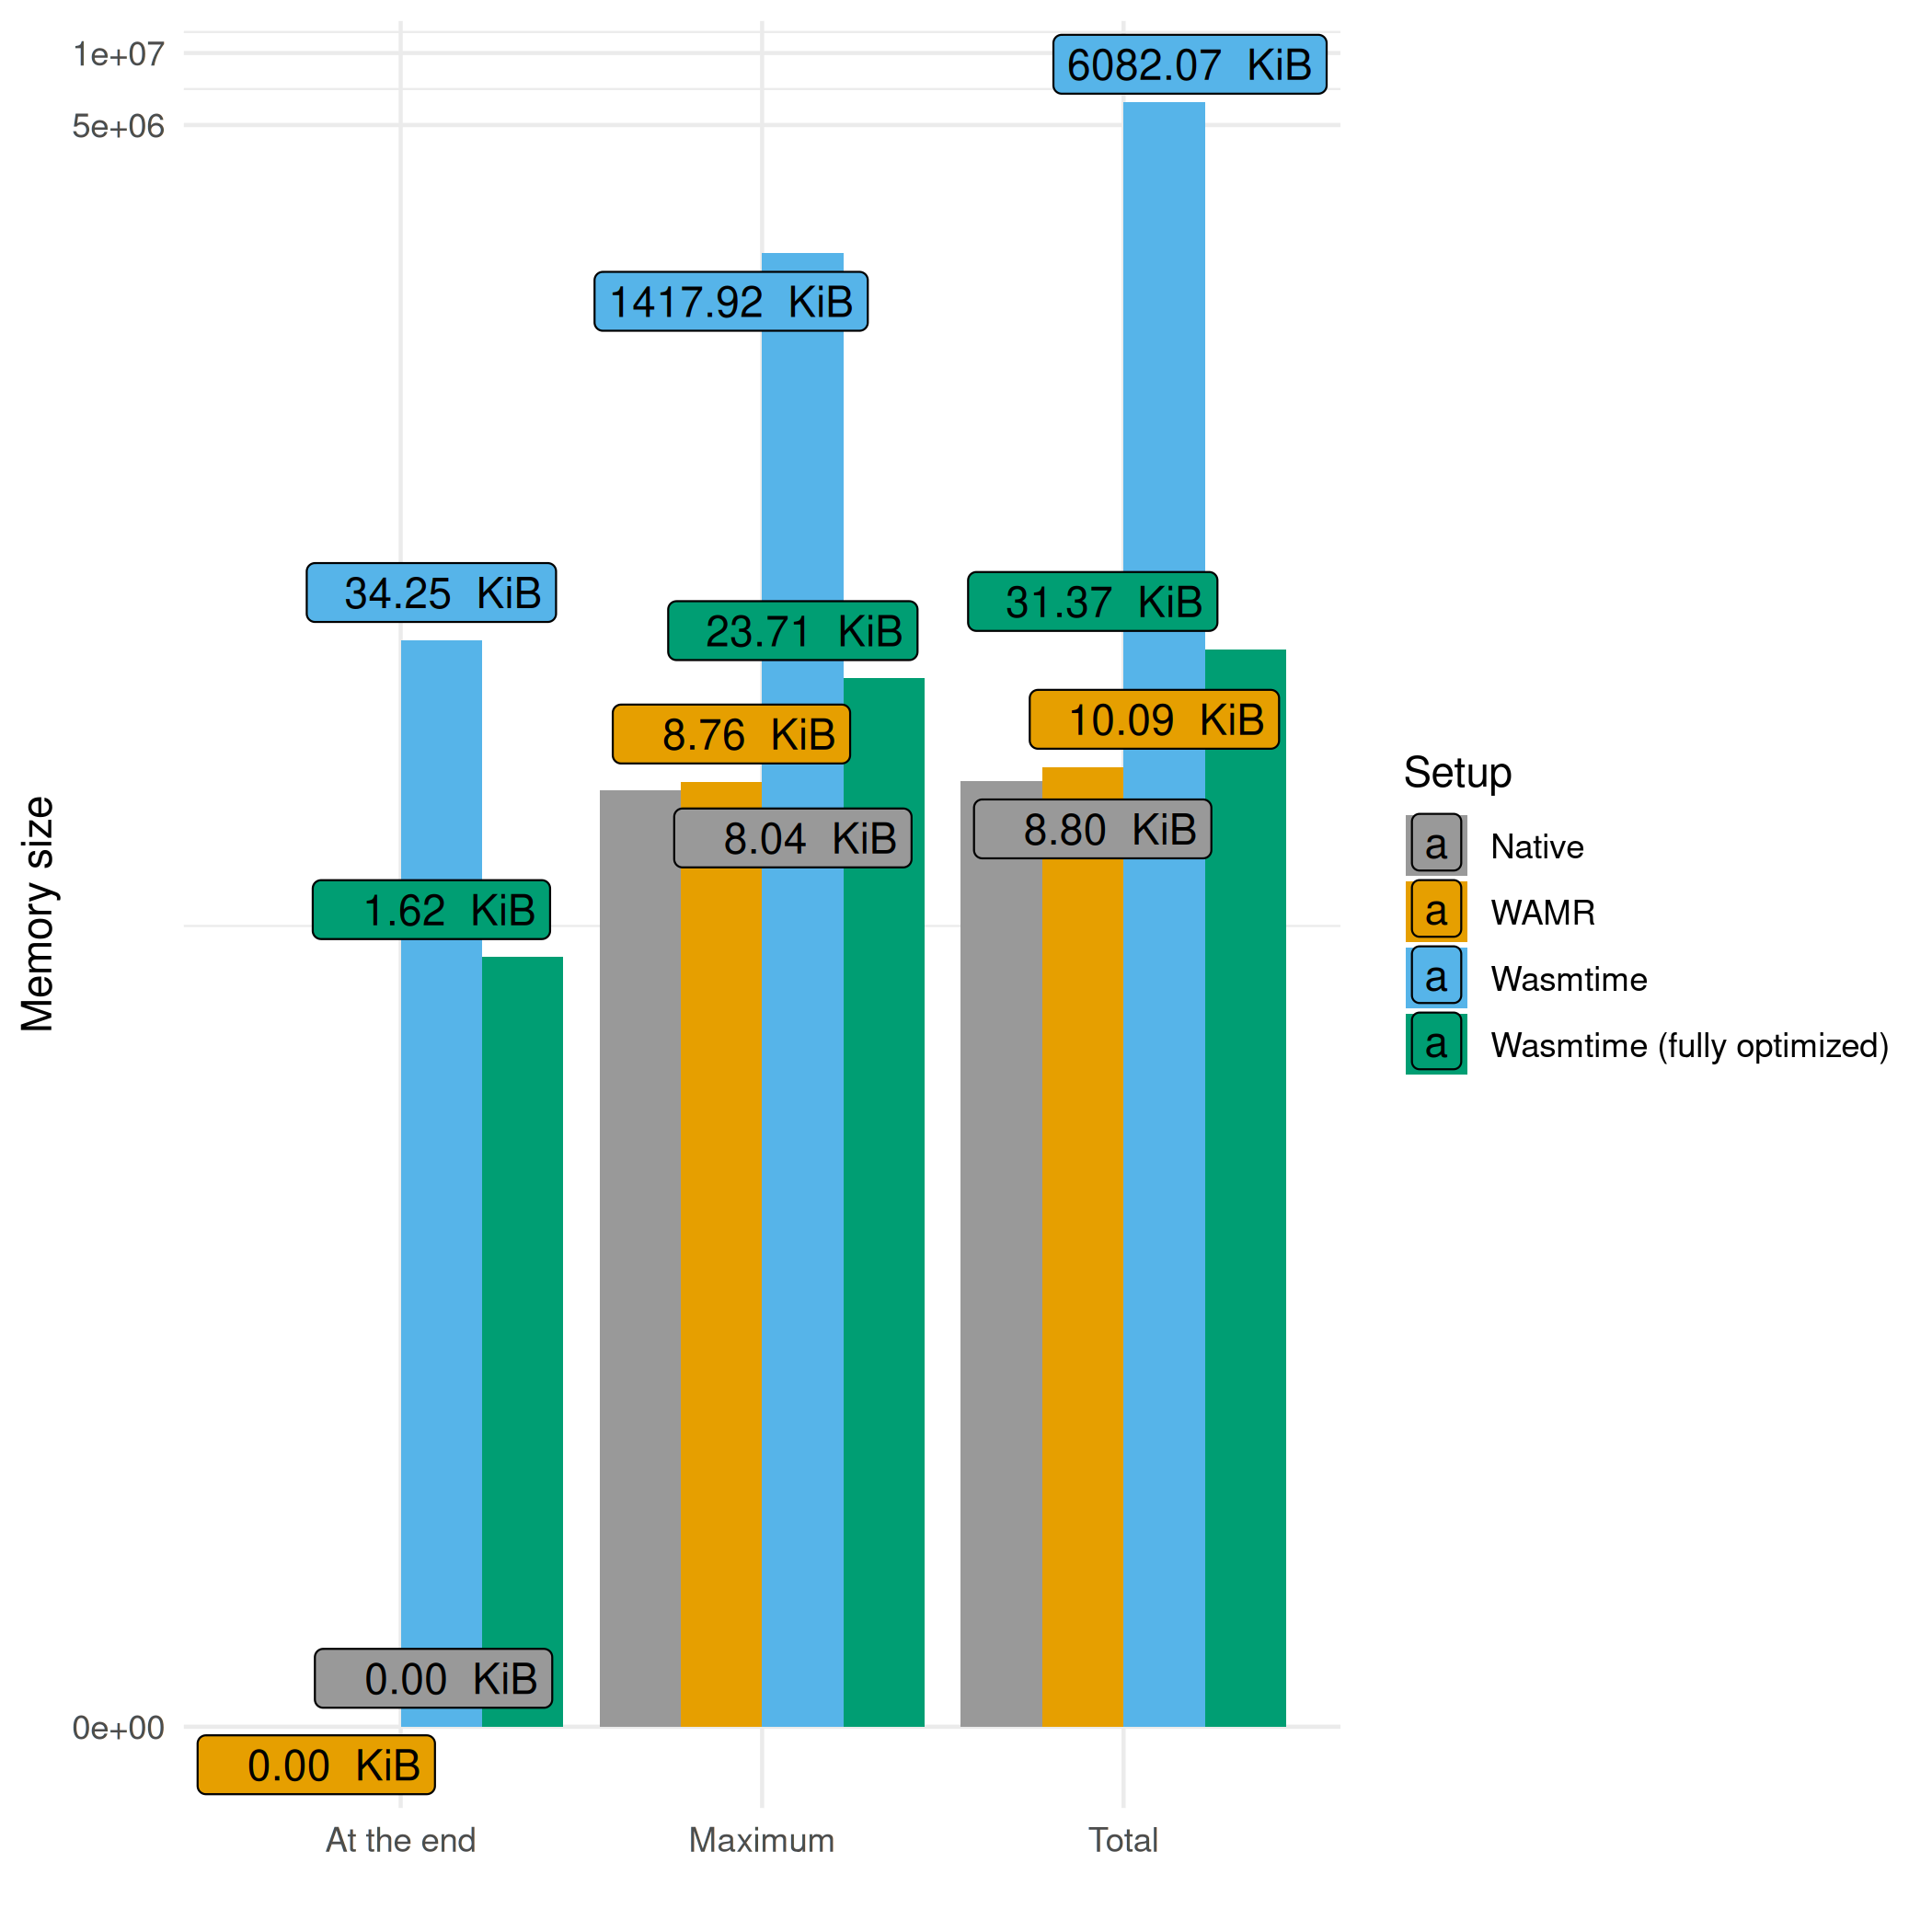
\includegraphics[width=0.5\textwidth]{figures/display_memory}
  \caption{Used memory size when writing to the display.}
\end{figure}

\begin{table}[h]
	\centering
	\captionsetup{justification=centering}
	% \label{tab:criteria}
	\begin{tabular}{l c c c}
		\toprule
                  & Total & Maximum & At the end \\ \midrule
      Native    & 8.8 KiB & 8.4 KiB & 0 B \\
      Wasmtime  &  5.94 MiB & 1.39 MiB & 34.25 KiB \\
      Wasmtime (fully optimized) & 31.17 KiB & 23.71 KiB & 1.62 KiB \\
      WAMR  &  10.9 KiB & 8.76 KiB & 0 B \\
		\bottomrule
	\end{tabular}
    \caption{Used memory for writing to the display}
\end{table}

\begin{table}[h]
	\centering
	\captionsetup{justification=centering}
	% \label{tab:criteria}
	\begin{tabular}{l c c c}
		\toprule
                  & Total & Maximum & At the end \\ \midrule
      Native    & 1.24 KiB & 1.03 KiB & 1 KiB \\
      Wasmtime  & 24.67 MiB & 2.66 MiB & 34.25 KiB \\
      Wasmtime (fully optimized) &  37.19 KiB & 29.58 KiB & 1.62 KiB \\
		\bottomrule
	\end{tabular}
    \caption{Used memory for reading from the sensor}
\end{table}

When considering the memory usage, three phenomena are striking. First, the performed optimizations to make the Wasmtime implementation run faster also greatly benefit the memory usage. Second, WAMR has near-native memory usage, while Wasmtime uses nearly four times more memory when compared to the native version. Third and last, the memory usage of the fully optimized version of Wasmtime is fairly similar between writing to the display and reading from the sensor. This showcases a baseline amount of memory required to run the component model.

To conclude, both solutions for Wasmtime greatly benefitted from precompiling the Wasm binary. Furthermore, precompilation makes Wasmtime on par with WAMR and native time-wise, but Wasmtime still requires a substantial larger amount of memory to succesfully run.

\begin{sidewaysfigure}
  \begin{subfigure}{\linewidth}
    \centering
    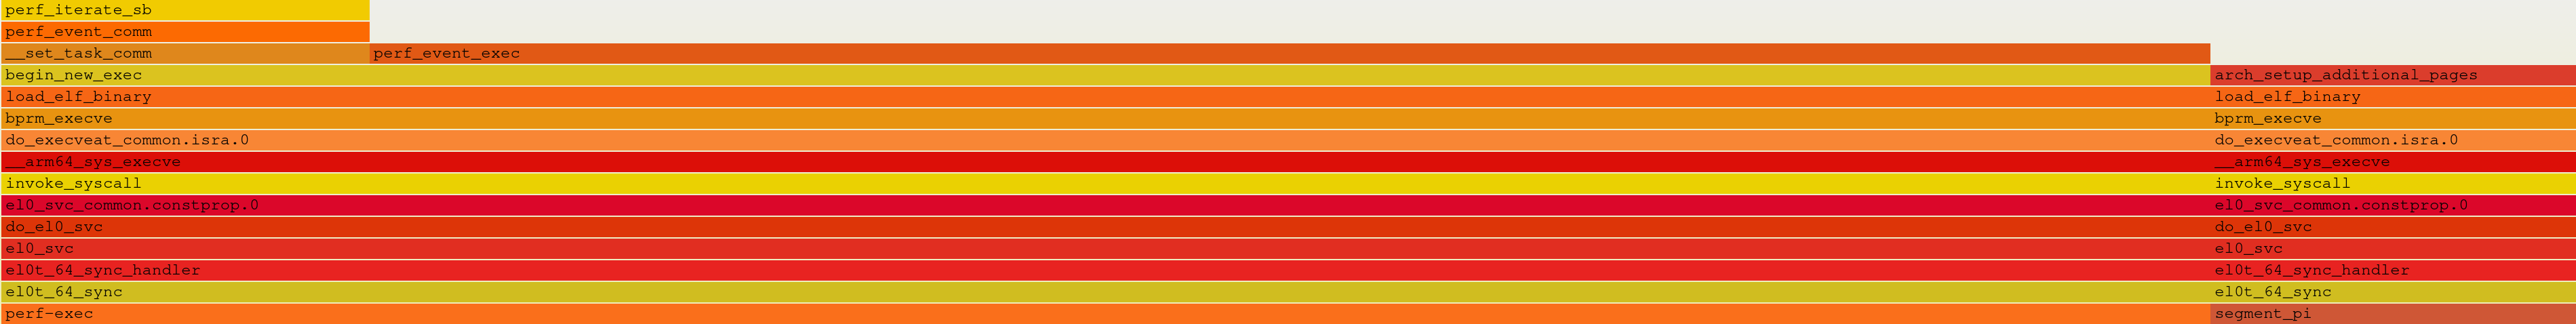
\includegraphics[width=\textwidth]{figures/native_led_flamegraph}
    \caption{Native}
    \label{fig:flamegraph:led:native}
  \end{subfigure}
  \begin{subfigure}{\linewidth}
    \centering
    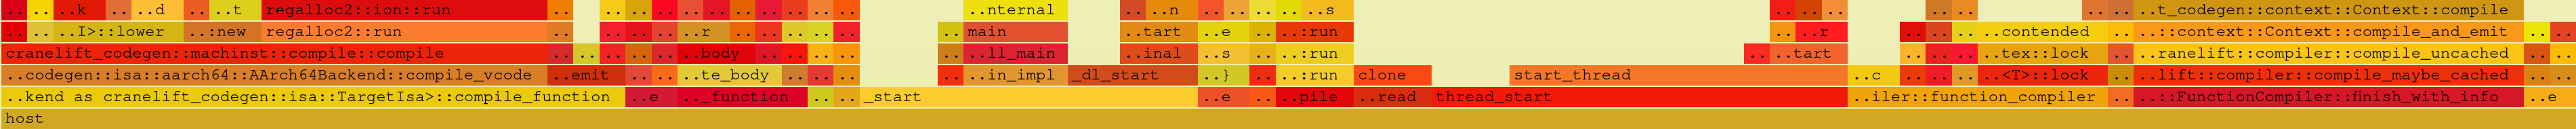
\includegraphics[width=\textwidth]{figures/wasmtime_flamegraph}
    \caption{Inside Wasmtime}
    \label{fig:flamegraph:wasmtime}
  \end{subfigure}
  \begin{subfigure}{\linewidth}
    \centering
    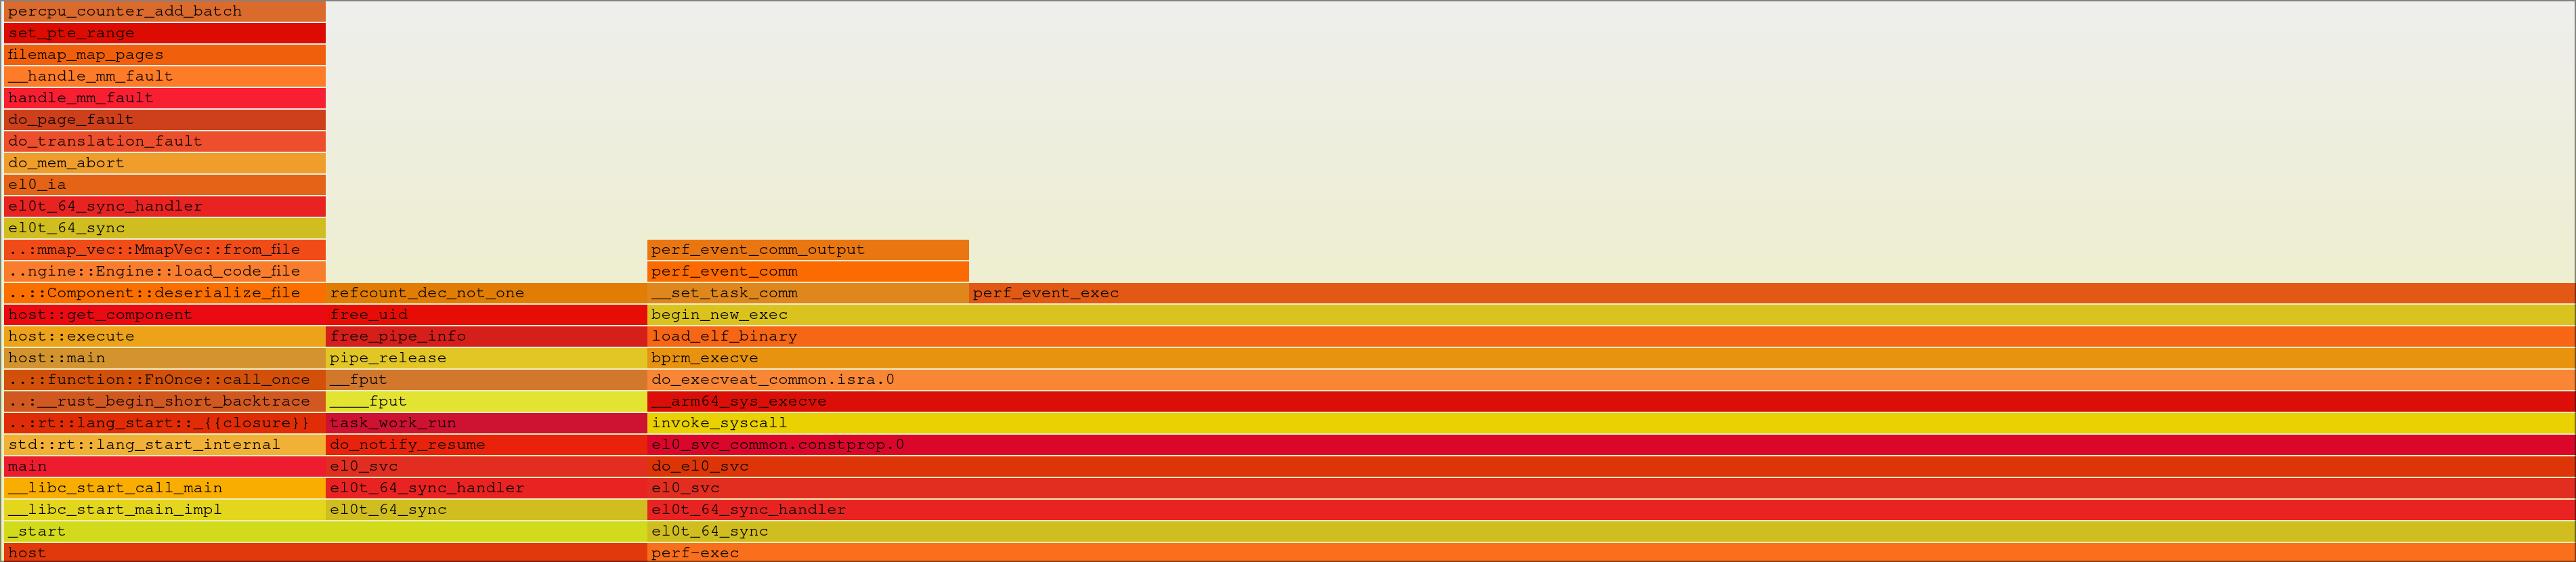
\includegraphics[width=\textwidth]{figures/optim_led_flamegraph}
    \caption{Inside Wasmtime (precompiled binary \& without command world)}
    \label{fig:flamegraph:led:compiled}
  \end{subfigure}
  \begin{subfigure}{\linewidth}
    \centering
    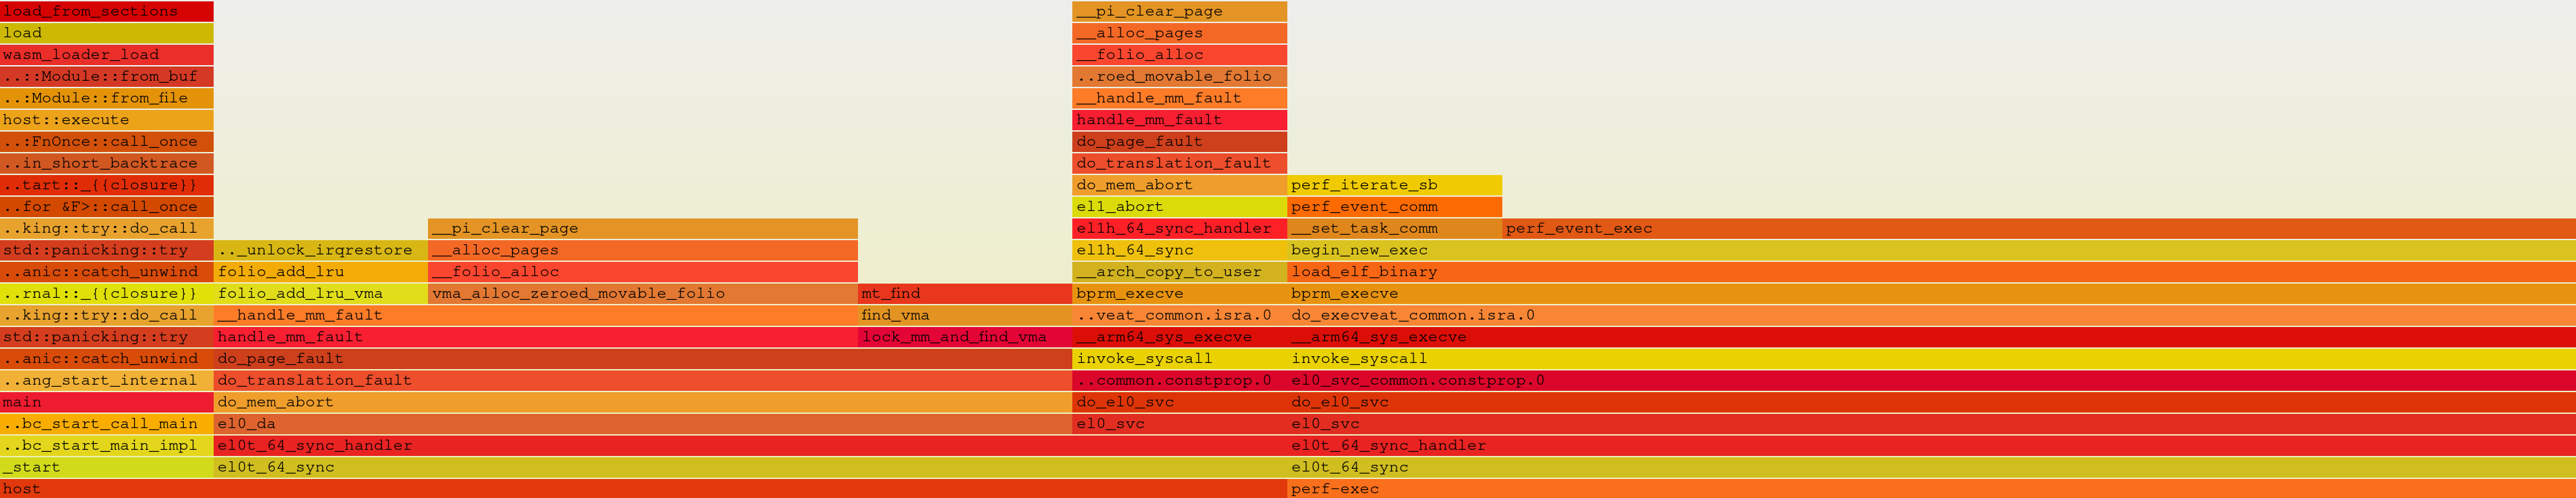
\includegraphics[width=\textwidth]{figures/wamr_led_flamegraph}
    \caption{Inside WAMR}
    \label{fig:flamegraph:led:wamr}
  \end{subfigure}
  \caption{Flamegraphs of writing to the display}
\end{sidewaysfigure}

\begin{sidewaysfigure}
  \centering
  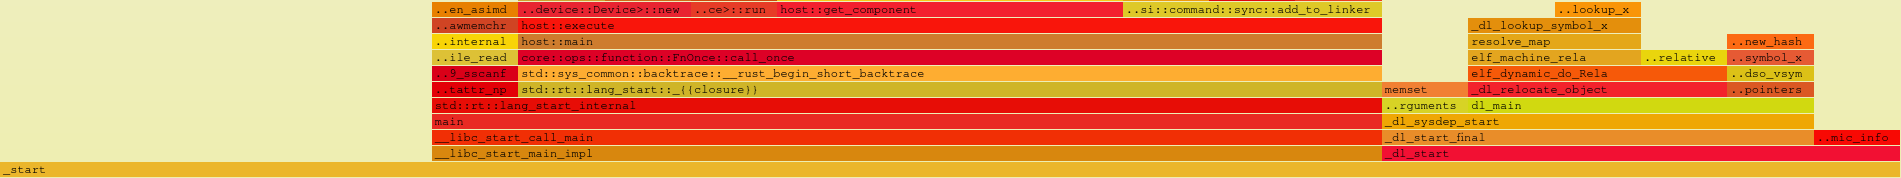
\includegraphics[width=\textwidth,keepaspectratio]{figures/compiled_sensor_flamegraph}
  \caption{Flamegraph of reading the sensor inside Wasmtime with a precompiled component.}
  \label{fig:flamegraph:sensor}
\end{sidewaysfigure}

